\appendix

\pagenumbering{Alph}
\renewcommand{\thechapter}{\Alph{chapter}}
\renewcommand{\thesection}{\Roman{section}}
\renewcommand{\thesubsection}{\Roman{section}}

\chapter{Anhang}
\label{appendix:annex}

\section{Bilder}
\begin{wrapfigure}{l}{\textwidth}
  \begin{centering}
    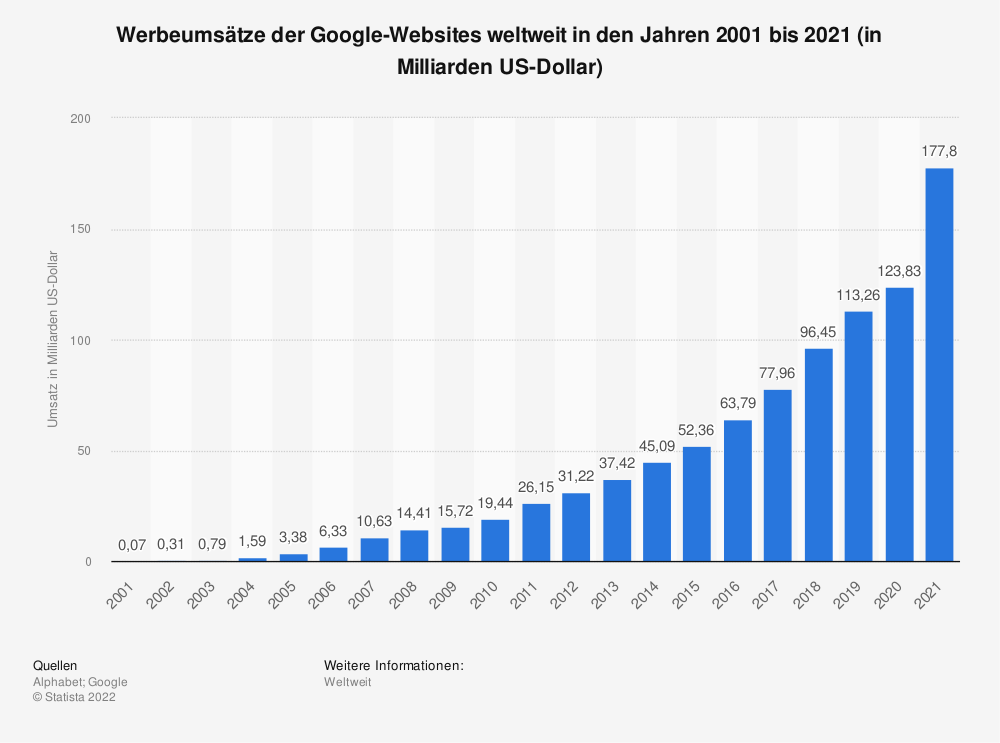
\includegraphics[width=.8\textwidth]{figures/appendix/werbeumsatz.png}
    \caption{Werbeumsätze Google Websites \cite{alphabet2022}}
    \label{fig:werbeumsatz}
  \end{centering}
\end{wrapfigure}

\begin{wrapfigure}{r}{\textwidth}
  \begin{centering}
    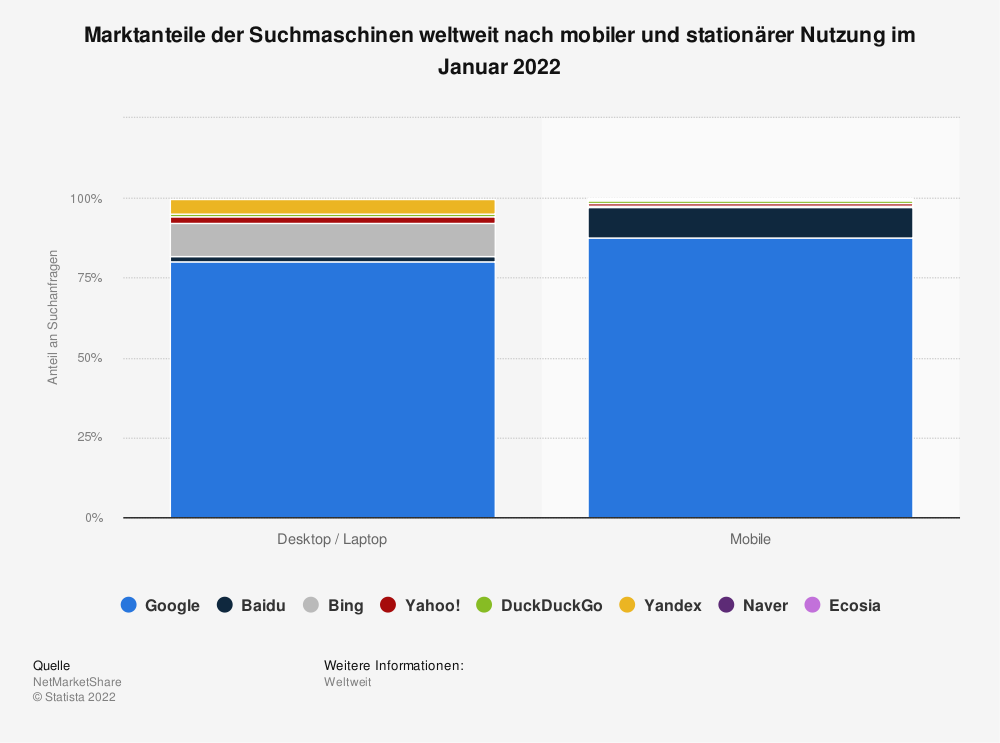
\includegraphics[width=.8\textwidth]{figures/appendix/marketshare.png}
    \caption{Marktanteil Google \cite{netmarketshare2022}}
    \label{fig:marketshare}
  \end{centering}
\end{wrapfigure}

\begin{wrapfigure}{r}{\textwidth}
  \begin{centering}
    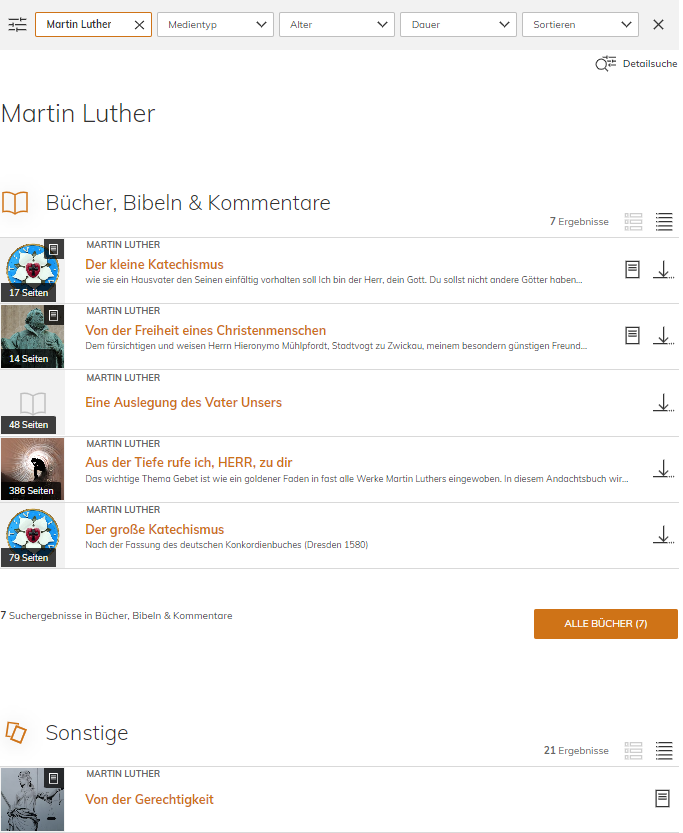
\includegraphics[width=.8\textwidth]{figures/appendix/crossloadSuche.png}
    \caption{Crossload \cite{pfleiderer2022}}
    \label{fig:crossloadSuche}
  \end{centering}
\end{wrapfigure}


% 2 Images on one page
% \begin{figure}
%   \includegraphics[width=\textwidth]{figures/appendix/IMAGE.png}
%   \caption{\label{fig:IMAGE} TITLE \cite{CITATION}}
%   \includegraphics[width=\textwidth]{figures/appendix/IMAGE.png}
%   \caption{\label{fig:IMAGE} TITLE \cite{CITATION}}
% \end{figure}

% 1 Images per page
% \begin{figure}
%   \includegraphics[width=\textwidth]{figures/appendix/IMAGE.png}
%   \caption{\label{fig:IMAGE} TITLE \cite{CITATION}}
% \begin{figure}
% \end{figure}
%   \includegraphics[width=\textwidth]{figures/appendix/IMAGE.png}
%   \caption{\label{fig:IMAGE} TITLE \cite{CITATION}}
% \end{figure}
